% This must be in the first 5 lines to tell arXiv to use pdfLaTeX, which is strongly recommended.
\pdfoutput=1
% In particular, the hyperref package requires pdfLaTeX in order to break URLs across lines.

\documentclass[11pt]{article}

% \usepackage[review]{acl}
\usepackage{acl}
\usepackage{times}
\usepackage{latexsym}
\usepackage[T1]{fontenc}
\usepackage[utf8]{inputenc}
\usepackage{microtype}
\usepackage{inconsolata}
\usepackage{booktabs}
\usepackage{multirow}
\usepackage{subfiles}
\usepackage{graphicx}
\usepackage{colortbl}

% Commands 
\newcommand{\draftonly}[1]{#1}
\newcommand{\draftcomment}[3]{\draftonly{\textcolor{#2}{[#3]{$_{\textsc{#1}}$}}}}
\newcommand{\lj}[1]{\draftcomment{Lj}{red}{#1}}
\newcommand{\libertus}{\textsc{LiBERTus}}
% \newcommand{\teamname}{Team 21a}
% \newcommand{\githuburl}{\url{https://anonymous.4open.science/r/sigtyp-1F05/}}
\newcommand{\teamname}{Allen AI}
\newcommand{\githuburl}{\url{https://github.com/ljvmiranda921/LiBERTus}}

\title{Allen Institute for AI @ SIGTYP 2024 Shared Task on Word Embedding Evaluation for Ancient and Historical Languages}

\author{Lester James V. Miranda \\
  Allen Institute for Artificial Intelligence \\
  \texttt{ljm@allenai.org} \\
}

\begin{document}

\maketitle

\begin{abstract}
  In this paper, we describe \teamname{}'s submission to the constrained track of the SIGTYP 2024 Shared Task.
  Using only the data provided by the organizers, we pretrained a transformer-based multilingual model, then finetuned it on the Universal Dependencies (UD) annotations of a given language for a downstream task.
  Our systems achieved decent performance on the test set, yet struggles with subtoken tags in multiword expressions as seen in \textsc{cop} and \textsc{hbo}.
  On the validation set, we obtained $\geq$70\% F1-score on most language-task pairs.
  We also explored the cross-lingual capability of our trained models.
  This paper highlights our pretraining and finetuning process, and our findings from our internal evaluations.
\end{abstract}

\section{Introduction}
This paper describes \teamname{}'s submission to the \textit{constrained} track of the SIGTYP 2024 Shared Task on Word Embedding Evaluation for Ancient and Historical Languages.
The constrained track requires participants to build a system for three linguistic tasks\textemdash parts-of-speech (POS) tagging, morphological annotation, and lemmatisation\textemdash using only the corpora provided by the organizers \cite{dereza-etal-2024-findings}.

The dataset contains Universal Dependencies v2.12 data \cite{zeman-etal-2023-universal} in eleven languages with Old Hungarian codices from MGTSZ.



Our general approach involves pretraining a transformer-based multilingual model on the shared task dataset \citep{dereza-etal-2024-findings}, and then finetuning the pretrained model using the Universal Dependencies (UD) annotations of each language.
Throughout this paper, we will refer to the pretrained model as \libertus{}.
We also explored data sampling and augmentation techniques during the pretraining step to ensure better generalization performance.

Our systems achieved decent performance on the test set, yet struggles with subtoken tags in multiword expressions as seen in \textsc{cop} and \textsc{hbo}.
Table \ref{table:main_results} shows our systems' performance on the shared task test set.
On the validation set, we obtained $\geq$70\% F1-score for the majority of language-task pairs.

We detail our resource creation, model pretraining, and finetuning methodologies in this paper.
The source code for all experiments can be found on GitHub: \githuburl{}.

\subfile{tables/main_results.tex}

\section{Methodology}

\subsection{Model Pretraining}

The main purpose of pretraining is to obtain context-sensitive word embeddings that we will finetune further for each downstream task.
We approach this by training a multilingual language model akin to the XLM-RoBERTa \cite{conneau-etal-2020-unsupervised} and multilingual BERT \cite{devlin-etal-2019-bert} architectures.

\begin{figure}[t]
  \centering
  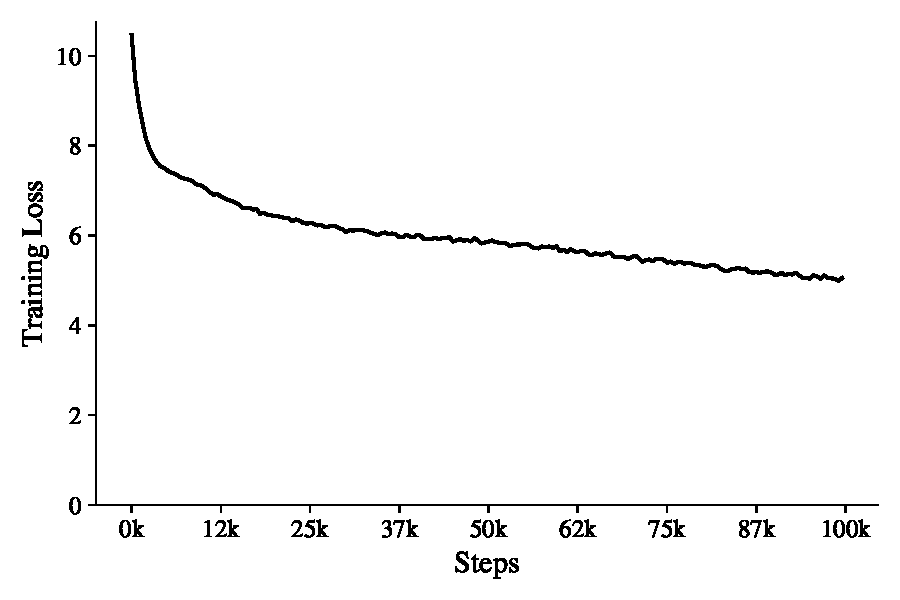
\includegraphics[width=0.5\textwidth]{figures/train_loss.pdf}
  \caption{Training loss curve for the 126M-parameter model after 100k steps.}
  \label{fig:training_curve}
\end{figure}

\paragraph{Preparing the pretraining corpora.}
We constructed the pretraining corpora using the annotated tokens of the shared task dataset.
Initially, we explored several data augmentation techniques to ensure that each language is properly represented based on the number of unique tokens.
However, we found pretraining to be unstable when we upsampled tokens to achieve the same count as \textsc{latm}, the most overrepresented language.
In the end, we found that leaving the token distribution as-is leads to more stable pretraining and lower validation scores.

\paragraph{Pretraining the base model.}
Using the pretraining corpora, we trained a model with 126M parameters that will serve as a base for finetuning downstream tasks.
\libertus{} follows RoBERTa's pretraining architecture \cite{liu-etal-2019-roberta} and takes inspiration from \citet{conneau-etal-2020-unsupervised}'s work on scaling BERT models to multiple languages.

\subfile{tables/pretrain_hyperparams.tex}

Our hyperparameter choices closely resemble that of the original RoBERTa implementation as seen in Table \ref{table:pretrain_hyperparams}.
We also trained the same BPE tokenizer \citep{sennrich-etal-2016-neural} using the constructed corpora.
During model pretraining, we used the AdamW optimizer with $\beta_2$=0.98 and a weight decay of 0.01.
The base model underwent training for 100k steps with a learning rate of 2e-4.
We used a learning rate scheduler that linearly warms up during the first 12k steps of the training process, then linearly decays for the rest.
Figure \ref{fig:training_curve} shows the training curve.

\subsection{Model Finetuning}

For each language, we finetuned a multitask model using spaCy \cite{honnibal-etal-2020-spacy}.
We used spaCy's tokenization rules for the majority of languages except for \textsc{lzh}, where we segmented on characters.
The final system consists of a parts-of-speech (POS) tagger, morphological analyzer, and lemmatizer.

\paragraph{Parts-of-speech (POS) tagger.}
We employed a standard classifier that predicts a vector of tag probabilities for each token.
Each POS tag is a unique class that we assign exclusively to a token.
We trained a model by taking the context-sensitive vectors from our pretrained embeddings, and passing it to a linear layer with a softmax activation.
The network is then optimized using a categorical cross-entropy loss.
For languages with subtokens such as \textsc{cop} and \textsc{hbo}, we merged each subtoken and used the full multi-word expression (MWE) during training.

\paragraph{Morphological analyzer.}
Similar to the POS tagger, we treat morphological annotation as a token classification task.
Instead of directly modeling each feature, we made every unique combination of morphological features as a class.
The limitation of this approach is that it can only predict combinations that were present in the training corpora.
Similar to the POS tagger, we merged each subtoken for every multi-word expression (MWE) during training.

\begin{figure*}[t]
  \centering
  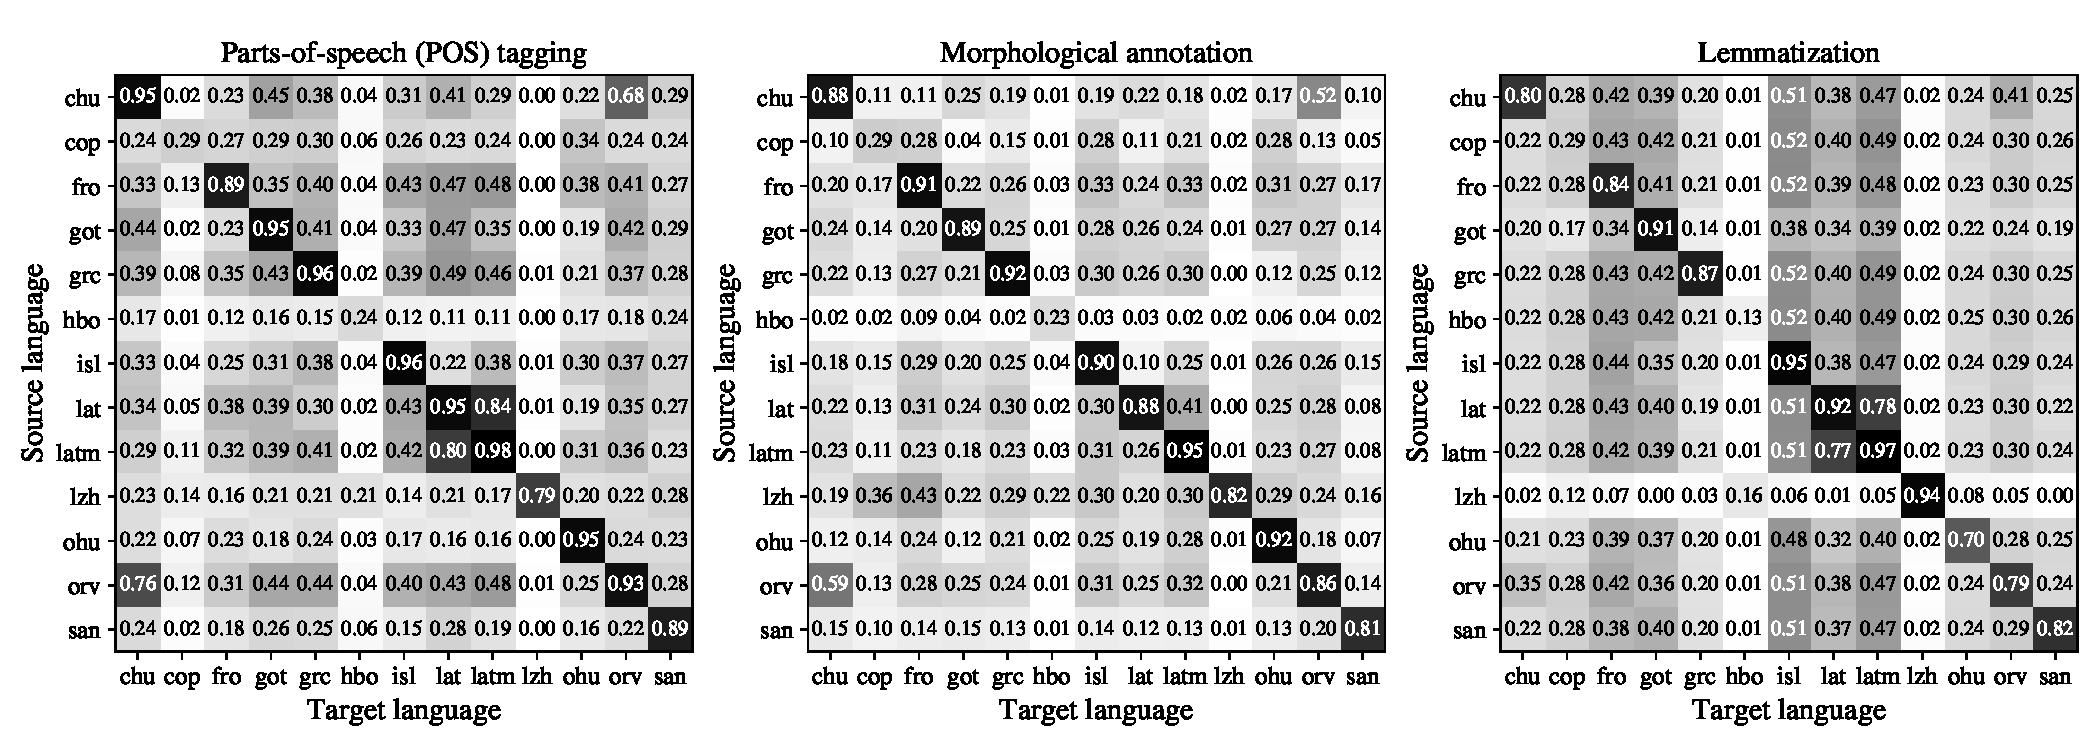
\includegraphics[width=\textwidth]{figures/cross_lingual.pdf}
  \caption{Cross-lingual evaluation given a monolingual model from one language and a validation set in another.}
  \label{fig:cross_lingual}
\end{figure*}


\paragraph{Lemmatizer.}
We trained a neural-based edit tree lemmatizer \cite{muller-etal-2015-joint} by first extracting an edit tree for each token-lemma pair.
Because this process can result to hundreds of edit trees, we treat the problem of picking the correct tree as a classification task.
Here, each unique tree serves as a class and we compute a probability distribution over all trees for a given token.
To obtain the most probable tree, we passed the context-sensitive embeddings from our pretrained model to a softmax layer and trained the network with a cross-entropy loss objective.
We set the minimum frequency of an edit tree to 3, and used the surface form of the token as a backoff when no applicable edit tree is found.
Finally, we ensured that the lemmatizer checks at least a single tree before resorting to backoff.

\paragraph{Finetuning the pipelines.} We trained each component of the system in parallel, although the final ``pipeline'' assembles them together using the spaCy framework.
For all components, the pretrained embeddings are passed on to linear layer with softmax activation.
Sometimes, the tokenization from the multilingual model does not align one-to-one with spaCy's tokenization.
In such case, we use a pooling layer that computes the average of each feature to obtain a single vector per spaCy token.

During finetuning, we used the Adam optimizer with $\beta_1$=0.9, $\beta_2$=0.999 and a learning rate of $0.001$.
The learning rate warms up linearly for the first 250 steps, and then decays afterwards.

\section{Results}

Table \ref{table:main_results} shows the test scores for the shared task.
Our systems obtained decent performance for the majority of language-task pairs.
In the following sections, we will outline our internal evaluations and benchmarking experiments.

\subsection{Performance on the validation set}

\subfile{tables/validation_results.tex}

Table \ref{table:validation_results} shows the validation scores of our finetuned models.
We achieved $\geq$70\% performance in most language-task pairs.
The top performers, calculated by taking the average across all tasks, are \textsc{latm} (0.968), \textsc{isl} (0.938), and \textsc{lat} (0.918),
whereas the bottom performers are \textsc{cop} (0.849), \textsc{san} (0.839), and \textsc{hbo} (0.468).

Compared to our validation scores, our leaderboard scores on \textsc{cop} and \textsc{hbo} are poor.
This performance is due to our models being unable to accurately predict subtoken information as it has only seen the full MWE during training.
In order to align our tokenization with the shared task's validation script in Codalab, we substituted each MWE with its subtokens resulting to potentially incomprehensible text.
Finally, for empty tokens such as previously found in \textsc{orv}, we added a rule in our system to produce empty predictions.\footnote[1]{This problem was initially caused by missing brackets in the reference annotations. We used the correct tokens for \textsc{orv} in the final submission.}

\subsection{Evaluating cross-lingual capabilities}
\label{sec:results_crosslingual}

To test the cross-lingual capability of a language, we evaluated its finetuned model to the validation set of another.
Figure \ref{fig:cross_lingual} shows the results.

We found that it is possible to adapt a language onto another for morphological annotation and lemmatization.
However, this does not extend to its morphology, as the validation set performs best only in the language it was trained on.

Some target languages tend to be cross-lingually receptive on lemmatization, i.e., many source languages can perform decently when applied to them.
This observation is true for \textsc{fro}, \textsc{got}, \textsc{isl}, \textsc{lat}, and \textsc{latm}.
Finally, there is also good cross-lingual compatibility between \textsc{lat} and \textsc{latm}\textemdash which is expected because they came from similar roots.

\section{Conclusion}

This paper describes Team \teamname{}'s system: a pretrained multilingual model (\libertus{}) finetuned on different languages for each downstream task.
Our system obtained decent performance for the majority of language-task pairs.
However, due to our training paradigm, it struggles annotating subtokens of multiword expressions.
Nevertheless, our validation scores are high ($\geq$70\% F1-score) for the majority of language-task pairs.

We also evaluated each language's cross-lingual capability and showed that transfer learning is possible especially on lemmatization.
This approach can be a viable alternative on limited corpora.

Our training and benchmarking source code is on GitHub: \githuburl{}.
The pretrained multilingual model and finetuned pipelines are also available on HuggingFace.\footnote[2]{\url{https://huggingface.co/collections/ljvmiranda921/sigtyp2024-shared-task-models-65629ea0462e5ebcbf1a2133}}

\section*{Limitations}

\paragraph{Pretrained LM size.}
Due to compute constraints, we were only able to pretrain a model akin to the size of RoBERTa\textsubscript{base}.
We highly recommend pretraining a large \libertus{} model to obtain performance gains if the resource allows.

\paragraph{Pretraining data mix.}
In the end, we didn't employ any sampling strategy to balance the token distribution of different languages during pretraining.
We only tested simple up-/downsampling strategies and our experiments are limited to repeating available data.

\paragraph{Label combination as individual classes}
When training the morphologizer and POS tagger, we treated each feature and parts-of-speech combination as its own class instead of modeling them individually.
This limits our text classifier to only predicting combinations it has seen during the training process.

\paragraph{Subtoken performance for multiword expressions}
Our systems performed poorly on \textsc{cop} and \textsc{hbo} in the leaderboard due to how we trained our model.
Instead of showing subtokens, we used the full multi-word expression during training.

\bibliography{custom}

\appendix

\section{Appendix}
\label{sec:appendix}

\subsection{Different sampling strategies on pretraining validation performance}

We explored different sampling strategies and their effect on the pretraining validation loss curve as shown in Figure \ref{fig:effect_sampling}.
We ran the pretraining pipeline for 20k steps (one-fifths of the final hyperparameter value) and measured the validation loss.
The evaluation corpus was built from the validation set of the shared task, and we kept it the same throughout the experiment.
We tested the following sampling strategies:

\begin{itemize}
  \item \textbf{None:} we used the original dataset without any data sampling or augmentation.
  \item \textbf{Upsampling:} we upsampled each language to ensure that the number of their unique tokens is greater than or equal to the most dominant language.
  \item \textbf{Averaging:} we took the average number of unique tokens in the whole set and up-/downsampled each language based on this value.
\end{itemize}

\begin{figure}[t]
  \centering
  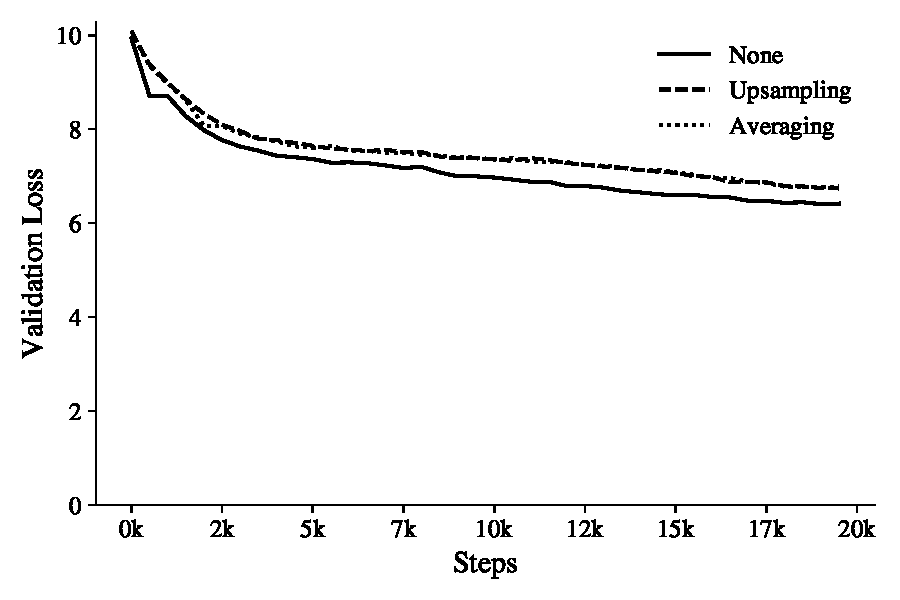
\includegraphics[width=0.5\textwidth]{figures/effect_sampling.pdf}
  \caption{Validation loss curve for different sampling strategies in 20k steps.}
  \label{fig:effect_sampling}
\end{figure}

Because any form of sampling resulted to unstable pretraining and higher validation loss, we decided to stick with the dataset's original data distribution.
We highly recommend exploring alternative data mixes to ensure that all languages will be represented while keeping the training process stable.

\subsection{Finetuning a model per language vs. monolithic system}

\begin{figure*}[t]
  \centering
  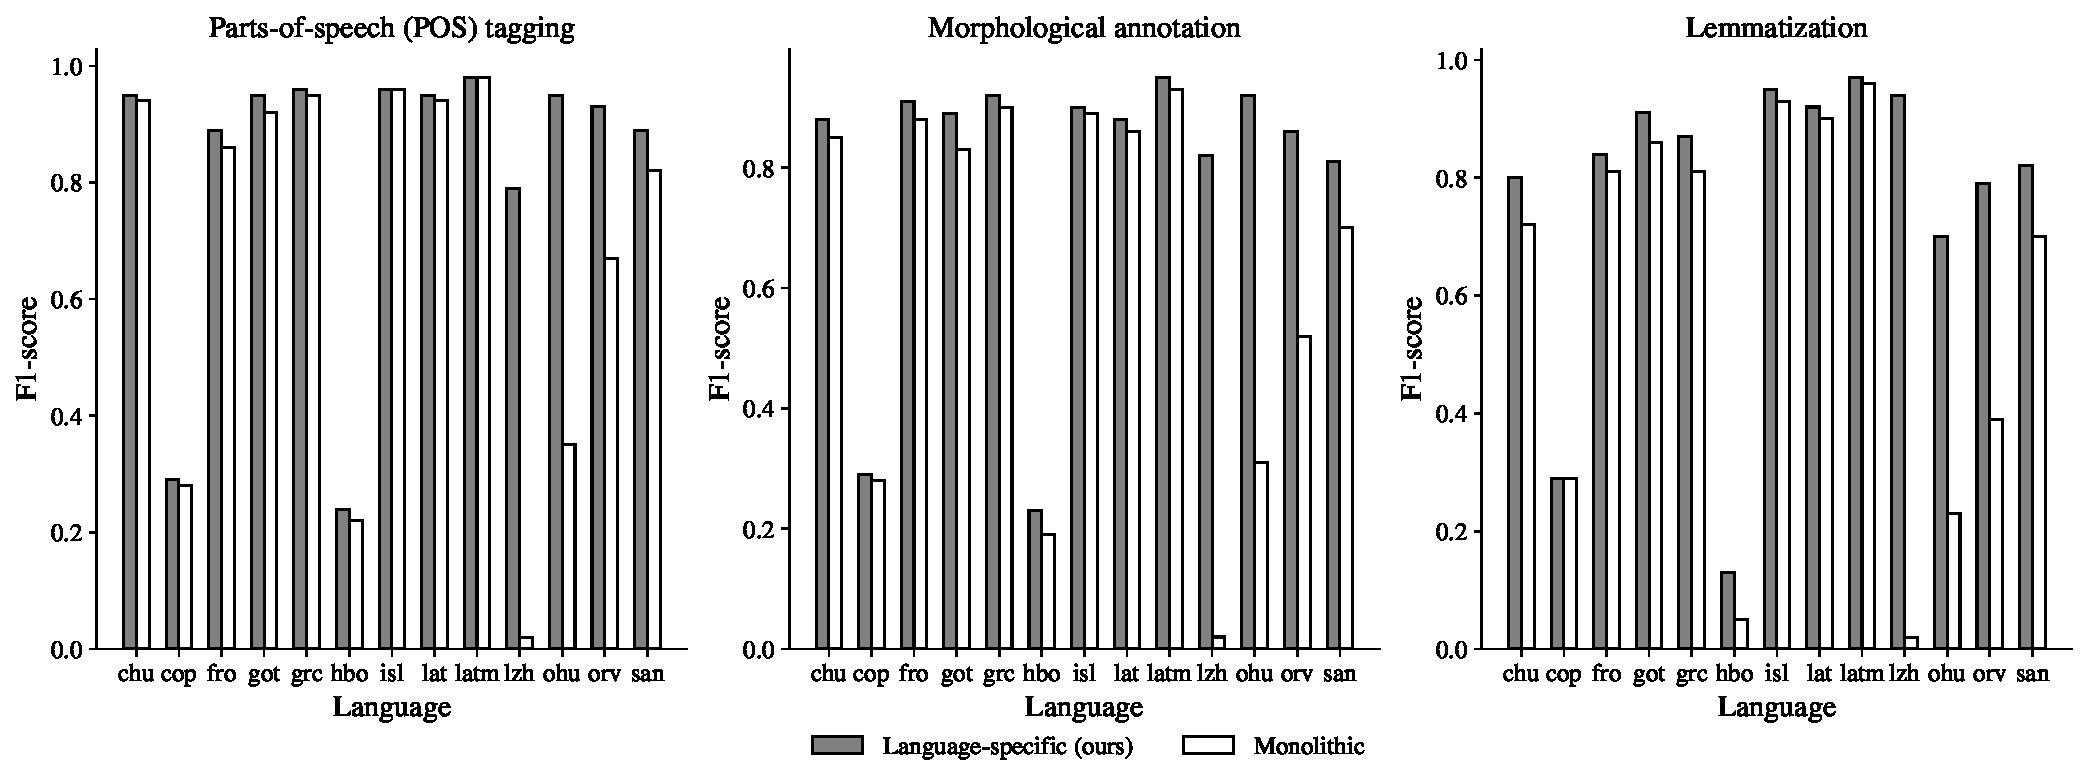
\includegraphics[width=0.95\textwidth]{figures/monolithic.pdf}
  \caption{Comparison between training language-specific models versus a single monolithic model as evaluated on the validation set.}
  \label{fig:monolithic}
\end{figure*}

We investigated if finetuning a model per language is more effective against a monolithic system, i.e., training on the full multilingual annotated corpora.
Here, we combined the training corpora for all languages, then shuffled them before batching.
The merged dataset has 194,281 documents for training and 26,954 documents for validation.
This means that the downstream model sees a language mix per training epoch.

As shown in Figure \ref{fig:monolithic}, finetuning a model per language still yields the best results.
One advantage of language-specific models is that we were able to set a different tokenizer per language\textemdash enabling us to get decent scores on \textsc{lzh}.
Training the monolithic model is also sensitive to the training data distribution, as shown by the disparity in performance between majority languages (\textsc{latm}, \textsc{lat}) and minority ones (\textsc{ohu}, \textsc{orv}, \textsc{san}).
Due to these findings, we decided to train multiple models for our final system.

\subsection{Alternative approach\textemdash multi-hash embeddings}

\begin{figure*}[t]
  \centering
  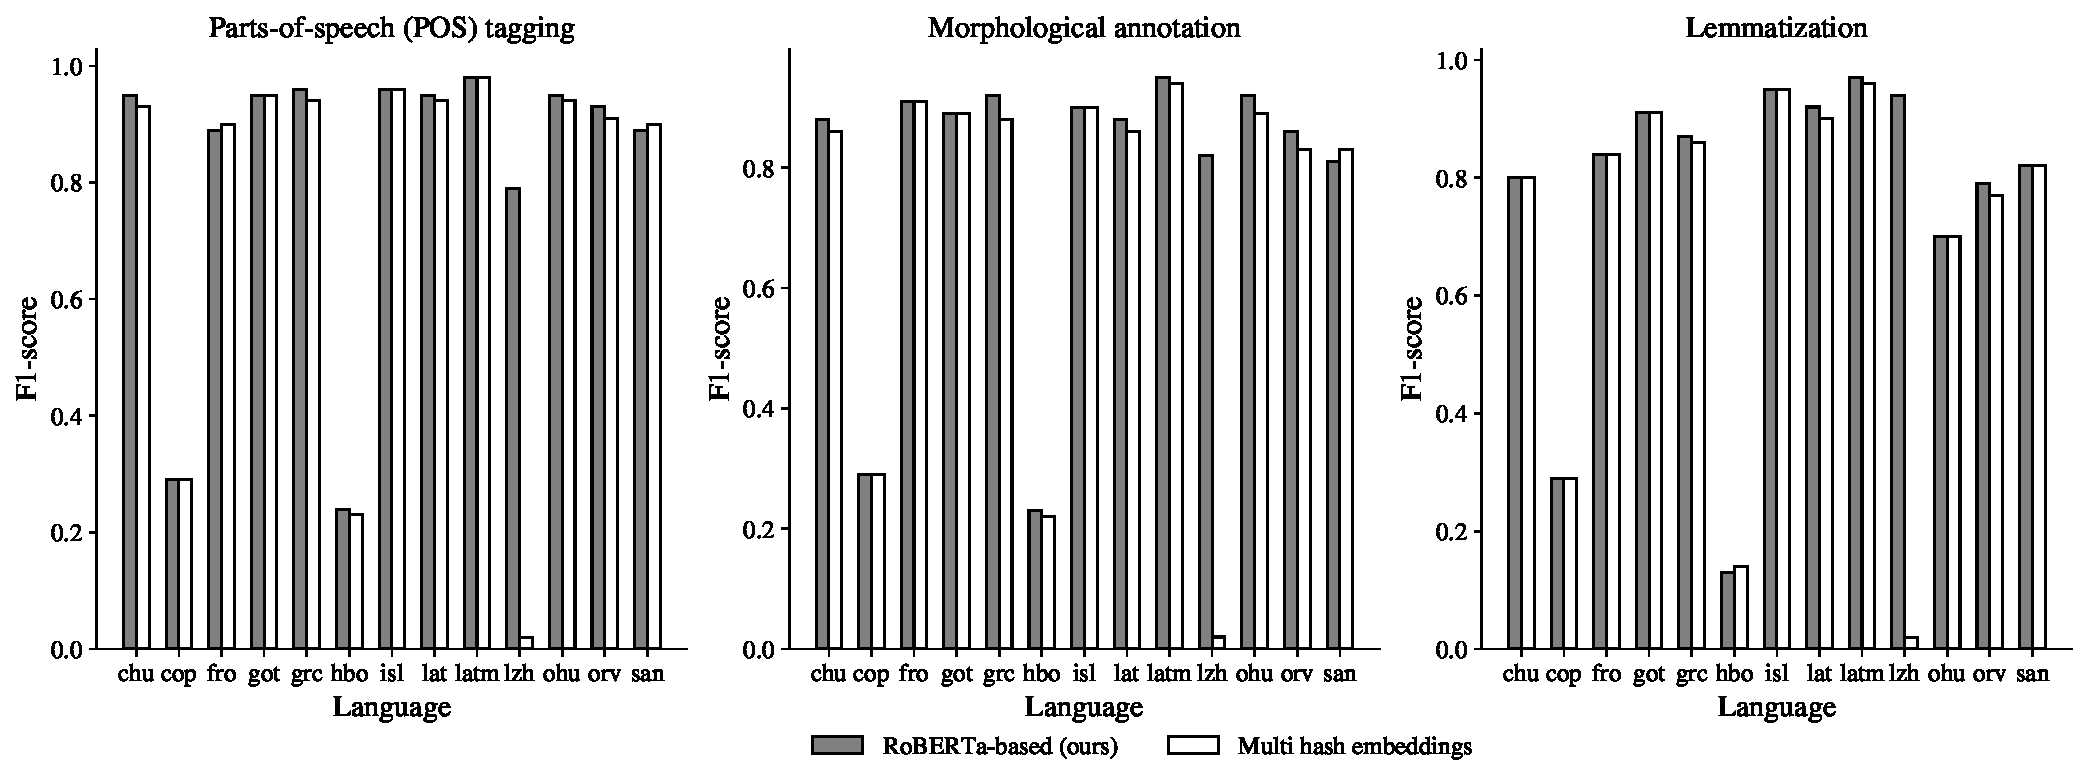
\includegraphics[width=0.95\textwidth]{figures/hashembed.pdf}
  \caption{Comparison between a RoBERTa-based pretrained model and multi-hash embeddings \cite{miranda-etal-2022-multi} as evaluated on the validation set.}
  \label{fig:hashembed}
\end{figure*}

We considered using multi-hash embeddings \cite{miranda-etal-2022-multi} as an alternative approach.
Instead of pretraining, these embeddings use orthographic features (e.g., prefix, suffix, norm, shape) to create a word vector table.
This approach also applies the hashing trick, inspired by Bloom filters \cite{bloom-1970-space}, to decrease the vector table's memory footprint.

Figure \ref{fig:hashembed} shows the results in comparison to our final system.
It is notable that simple orthographic features are competitive with our transformer-based model.
However, we chose to submit the transformer-based pipeline as our final system because it still outperforms the multi-hash embed method in the majority of our language-task pairs.
We still recommend investigating this approach further because the hash-embed method has noticeable efficiency gains in terms of model size.

\end{document}
